\setcounter{chapter}{15}
\chapter{Piles}

\section{La pile, un transfert d'électrons}
\subsection{Un exemple de réaction d'oxydo-réduction}
\subsection*{Expérience :}

\begin{figure}[h]
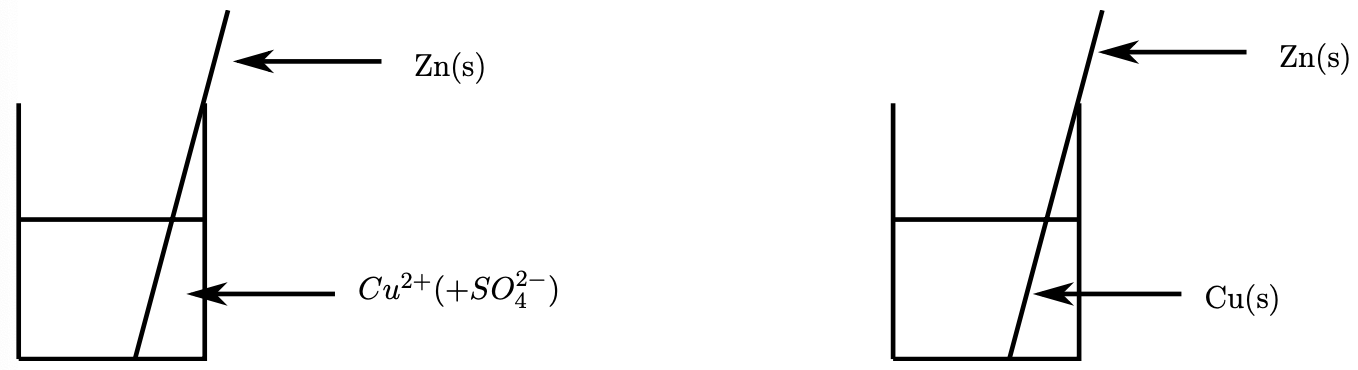
\includegraphics[scale=0.5]{figures/evolution/pile}
\end{figure}

\subsection*{Interprétation :}
On observe l'apparition de \trou{cuivre} sur la plaque de zinc. La réaction qui a eu lieu est donc :\\
\trou{$Cu^{2+}(aq) + 2e-=Cu(s)$}\\
D'où ces deux électrons peuvent-ils venir ?
Les deux électrons ont été cédés par \trou{le zinc : $Zn(s)=Zn^{2+}(aq) + 2e-$}\\
\trou{Donc, les deux électrons cédés par le zinc ont été captés par les ions $Cu^{2+}$}\\
On obtient donc l'équation de la réaction suivante :\\
\trou{$Zn(s)+Cu^{2+}(aq) \longrightarrow Zn^{2+}(aq) + Cu(s)$}

\subsection{Détournement d'électrons, réalisation d'une pile}

\subsection*{Expérience}
\begin{figure}[h]
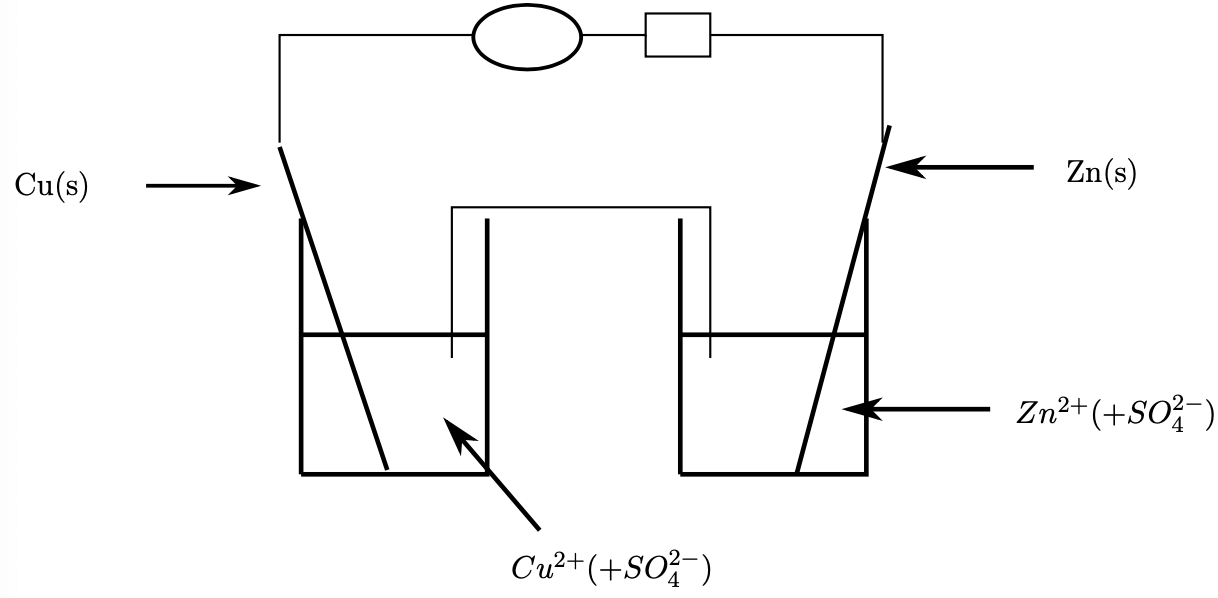
\includegraphics[scale=0.5]{figures/evolution/pile1}
\end{figure}



\subsection*{Observations}
On constate \trou{qu'un courant circule de la lame de cuivre vers la lame de zinc à l'extérieur de la pile.}\\
\subsection*{Interprétation}
Où est le pôle positif ? le pôle négatif ?\\
Noter sur le schéma ci-dessous le sens de déplacement des électrons ainsi que le sens conventionnel du courant.\\
Les électrons se déplacent-ils dans les solutions ?\\
\trou{Lorsque les électrons  créés par la réaction d'oxydation du zinc arrivent au niveau de la lame de cuivre, ils sont captés par les ions cuivre II pour former du cuivre.\\
Les électrons sont forcés à circuler à l'extérieur de la pile, ce qui génère un courant électrique, voilà pourquoi on peut évoquer un détournement d'électrons.}\\
\subsection*{Équation globale de la pile}
$Zn(s)+Cu^{2+}(aq) \longrightarrow Zn^{2+}(aq)+Cu(s)$
\subsection*{Rôle du pont salin}
Le pont salin assure la fermeture du circuit électrique. \\
Il n'y a pas d'électron dans le pont salin puisque les électrons ne se trouvent jamais en solution. Ce sont les ions qui conduisent le courant en solution.
Compléter sur le schéma le sens de déplacement des ions dans le pont salin.

\subsection*{Tension à vide}
\begin{minipage}{0,6\linewidth}
La tension mesurée aux bornes de la pile lorsqu'elle ne débite pas est appelée tension à vide. Elle est exprimée en volts.\\
Sur le schéma ci-contre, la borne V définit la borne positive de la pile
\end{minipage}
\begin{minipage}{0,4\linewidth}
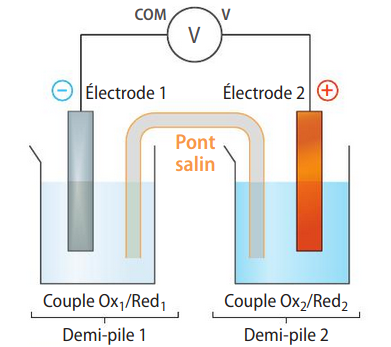
\includegraphics[scale=0.5]{figures/evolution/pile3}
\end{minipage}


\etiquetterouge{Important} Qu'est-ce qu'une pile usée ?\\
La pile en fonctionnement est un système hors équilibre, lorsqu'elle atteint \textbf{l'équilibre}, la réaction s'arrête, le courant ne circule plus, la pile est \textbf{usée}.

\subsection{Capacité d'une pile}

La capacité d'une pile, notée Q, est égale à la charge électrique qui circule pendant la durée totale de son fonctionnement, de l'état initial à l'usure complète.\\
Si l'on considère que l'intensité du courant I est constante pendant toute la durée de fonctionnement, alors on a :
\begin{center}
$Q=I\times \Delta t$ \\avec 
Q la capacité de la pile en coulombs(C)\\
I l'intensité du courant en ampères (A)\\
$\Delta t$ le durée de vie de la pile en secondes (s)
\end{center}
On peut également calculer la capacité d'une pile grâce à l'expression :
\begin{center}
$Q=Z\times x_f \times F$\\
Avec Z le nombre d'électrons échangés\\
$x_f$ l'avancement lorsque la pile a atteint son état d'équilibre, c'est à dire lorsqu'elle est usée\\
F la constante de faraday : $F=e\times N_a=\SI{9,65e4}{\coulomb\per\mole}$
\end{center}

\section{Quelques couples oxydant-réducteur usuels}
\blocgris{Demi-équations}{
Pour chacun des couples ci-dessous, écrire la demi-équation d'oxydo-réduction : 
\begin{itemize}
\item L'eau de javel est une solution d'ion hypochlorite $ClO^-$ oxydant du couple : $ClO^-/Cl^-$\\
\trou{$ClO^-+H_20+2e-=Cl^-+2HO^-$}
\item le dioxygène $O_2$ est l'oxydant du couple $O_2/H_2O$\\
\trou{$O_2+4e-+4H^+=2H_2O$}
\item le dichlore $Cl_2$ est l'oxydant du couple $Cl_2/Cl^-$\\
\trou{$Cl_2+2e-=2Cl^-$}
\item l'acide ascorbique ou vitamine C est le réducteur du couple $C_6H_6O_6/C_6H_8O_6$\\
\trou{$C_6H_6O_6 +2H^+  = C_6H_8O_6$}
\item le dihydrogène $H_2$ est le réducteur du couple $H^+/H_2$.\\
\trou{$2H^+ +2e-=H_2$}
\end{itemize}
}
\etiquette{Remarque}
Les éléments des deux premières colonnes du tableau périodique sont les éléments du bloc s. Ils ont tous un ou deux électrons sur leur couche externe. Ils sont donc susceptibles de les perdre, ce qui fait d'eau des \trou{réducteurs}

